\documentclass[a4paper,11pt]{article}
\usepackage{listings}
\usepackage{enumerate}
\usepackage{graphicx}
%\usepackage{hyperref}
\usepackage[font=small,labelfont=bf]{caption}
\usepackage{geometry}
\usepackage{wrapfig}
\usepackage{cite}
 


\title{House Price Prediction}
\date{March 28, 2019}
\author{Lucas Faijdherbe, Rico Mossinkoff, Ewoud Vermeij, Ruben van der Ham\\ and Harsh Khandelwal\\\\
Group 19\\
\small Machine Learning\\
\small Vrije Universiteit Amsterdam}

\begin{document}


\begin{titlepage}

\centering
\maketitle

\includegraphics[width=0.8\linewidth]{images/vulogo.png}
\pagenumbering{gobble} %pagenumbering OFF
\hfill
\\


\begin{abstract}
For this research project, 2 approaches are evaluated on their performance of predicting house prices given a set of features. Because the house prices are rising again after a period of decline, it is interesting to know the current value of your house. We are going to predict house prices for houses in Ames, Iowa.
    In this project we will evaluate two different approaches to estimate house prices: K-Nearest Neighbours and Linear Regression. We used a data set of the Kaggle competition “House Prices: Advanced Regression Techniques”. We performed some data analysis to make this data usable for testing. 
\end{abstract}
\end{titlepage}


%Table of contents page
%\tableofcontents
%\clearpage

\clearpage
\pagenumbering{arabic} %pagenumbering ON


\section{Introduction}
After the downfall of house prices in the Netherlands during the economic recession, prices are starting to rise again. In some areas the house prices are rising with a tremendous pace. A good example is Amsterdam, where house prices rose with a staggering 20\% in one year \cite{couzy_damen_2018}. Fluctuations in house prices are not only interesting for potential house owners, but also for investors, which are partial responsible for the upswing in house prices \cite{couzy_2018}. This makes house price prediction an interesting topic.\\

The data used for the training and testing of the prediction algorithms came from Kaggle.com from a competition called \textit{“House Prices: Advanced Regression Techniques"}. The dataset provided for this competition contains the features of residential homes of a Ames, a small town in Iowa, United States. It has to be noted that a potential model that is able to predict the house prices of this dataset is unlikely to have the same performance on a dataset of a different residential area. Nonetheless it is a great dataset to use for this research. The goal is to be able to have a model that can accurately predict the house prices for this dataset.\\

    There have been several approaches for predicting or evaluating house prices. The hedonic-based regression is an one approach. With hedonic-based methods, relationships between house prices and house characteristics are tried to be identified. This has been utilized in many reports \cite{adair_berry_mcgreal_1996, stevenson_2004, bin_2004}. Besides hedonic-based regression, there have been several approaches in the machine learning area. Interestingly we found that these approaches are not necessarily complex ones. Use of a decision tree is a relatively simple approach, but can get a descent squared error rate such as 0.885 \cite{fan_ong_koh_2006}. It is also shown that an algorithm like RIPPER, a rule-learning algorithm, can outperform slightly more complex algorithms such as Naïve Bayesian and AdaBoost \cite{park_bae_2015}. Therefore this report is focused more on investigating the performance among relatively simple algorithms. \\
 
The focus will be on two different machine learning techniques: linear regression and k-nearest neighbours. According to earlier research \cite{zhao_sun_wang_2014}, k-nearest neighbours (kNN) can have some promising results when it comes to house price prediction. For linear regression no relevant research was found, so this paper will try to investigate its performance. It is expected that kNN will be relatively accurate. To compare the results a baseline model is used. This baseline predicts every house price with the average of all house prices. The models laid out in this report should perform better than this baseline model, as the average will not give a very good prediction. \\

This following of the report is structured as follows. Section 2 will talk about the dataset analysis, and discuss the data preparation. Section 3 will discuss the models individually. Section 4 will present the experimental results and section 5 will conclude remarks on the results. 
s. 



\section{Data analysis and preparation}
%figuur heatmap
\begin{minipage}{1\linewidth}
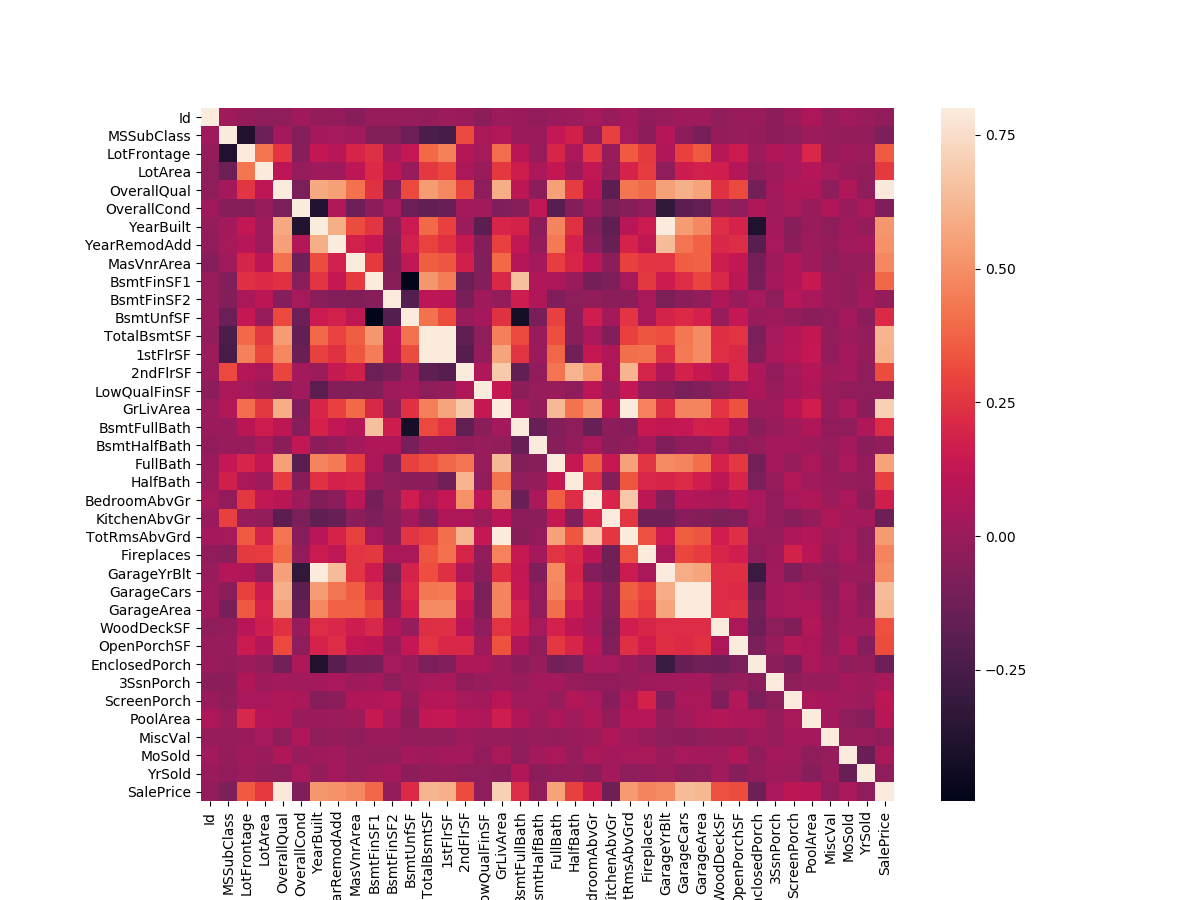
\includegraphics[width=\linewidth]{images/heatmap.png}
\captionof{figure}{}
\end{minipage}

In order to get the best performance from the machine learning models, the dataset features need to be analyzed and prepared such that the models can work with the data and will be able to make predictions based off of it.\\
The first section will take a closer look at all features to get a good understanding of how all data is distributed, how it is presented (numerical or categorical) and if any data is missing. The next section will elaborate on the data preparation decisions made in order to get the best results with the models.



\subsection{Data Analysis}

\begin{minipage}{0.6\linewidth}
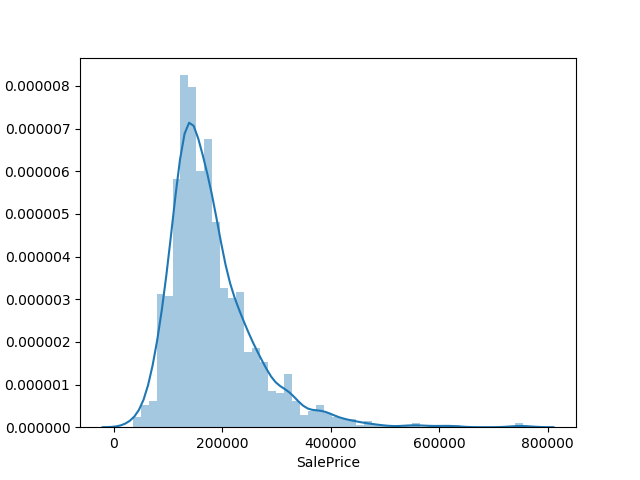
\includegraphics[width=\linewidth]{images/distribution.png}
\captionof{figure}{}
\end{minipage}
\begin{minipage}{0.39\linewidth}
The dataset provided through the Kaggle competition consists of 79 features describing the residential homes from Ames, Iowa. The Kaggle competition provided two datasets: one to train on and one to predict from. However, the prediction data set does not include the actual house prices. It is not possible to use this dataset, since there will be no way to check if the model prediction performed well on this data. Only the ‘train’ dataset will be used, which will be split randomly in a train and test set. This dataset consists of 1460 entries.
\end{minipage}
\\
\\
Since sale price is the target to predict, let us look how the sale price relates to other properties. Figure 2 is a distribution plot that shows that the sale price looks like a right skewed normal distribution. Most of the sale prices lie around 180.921 dollars. This is the mean of the data and this will be used for the baseline.\\

Figure 1 shows a heatmap which shows the correlation between 40 of the features, including the sale price. This can be very valuable information. Features with little or close to zero correlation with respect to the sale price could be left out from training a model, since they do not say much about the sale price. On the other side, features with high correlation with the sale price are valuable. Putting the emphasis on these features when training the models can be meaningful. \\


\begin{wraptable}{l}{0.5\linewidth}
\centering

\begin{tabular}{|c|c|}
\hline
\textbf{Feature} & \textbf{Percent missing} \\ \hline
PoolQC           & 0.995205                 \\ \hline
MiscFeature      & 0.963014                 \\ \hline
Alley            & 0.937671                 \\ \hline
Fence            & 0.807534                 \\ \hline
FireplaceQu      & 0.472603                 \\ \hline
LotFrontage      & 0.177397                 \\ \hline
GarageCond       & 0.055479                 \\ \hline
\end{tabular}


\captionof{figure}{}

\end{wraptable}

Figure 3 shows a table of the six features having the highest fraction of missing values. In some situations it can be in helpful to delete the rows containing missing value(s) for one or more features. In this situation, this is not a viable option since 99.5\% of the rows have no value for the pool quality.

\clearpage
\subsection{Data Preperation}
In order to make the data useable for the models, some enhancements need to be made. Since the sale price data was somewhat skewed, log transformation was performed in order to normalise it. For categorical features that missed entries (e.g. entries containing NA), the entries were filled. As an example, for the feature \textit{"central air conditioning"}, all the missing entries were assumed to a NO, since there are only two possibilities, a YES and a NO. Some categorical features containing numerical values were changed to numerical features. An example is garage quality, where the conditions ranged from poor to excellent. These can be easily changed into numerical features. However, these changes do not always work out well so in some cases the numerical features had to be changed back to categorical features.\\

Next, missing values for numerical features were handled by taking the mean of the feature as a replacement. The numerical features that were skewed were also log transformed, in order to normalize them. For categorical features one-hot coding was applied, in order to only have numerical features in the feature space. In the end, the correlation between features and sale price was plot again. The 80 highest correlated features with respect to the sale price were taken. The other features were discarded. These discarded features were the most ‘meaningless’, so the model should perform better since the decisions will be based on more highly correlated features. 


\clearpage
\section{Evaluated Models}
\subsection{Linear Models}
Linear Regression models all the input variables to the house price, and can make predictions based of this model. Linear Regression will try to find the best fitting line for the model. We performed data regularization to fit the model better. This is a technique to reduce the magnitude of the coefficients, in order to modularize the impact of some very high and sporadic coefficients on the model. Soothing the effect of outliers, through regularization, also helps to prevent overfitting.\\

Three variants of linear regression were performed. One with LASSO (LL(1)) \cite{fonti} regularization, one with Ridge (LL(2)) \cite{nie_huang_cai_ding} regularization, and one without any regularization. The LASSO (Least Absolute Shrinkage and Selection Operator) is a regression method that involves penalizing the absolute size of the regression coefficients. By constraining the sum of the absolute values of the estimates, some of the parameter estimates tend to be exactly zero. As the penalty gets larger, more estimates are shrunk towards zero. Ridge regression adds “squared magnitude” of coefficient as penalty term to the loss function.\\

LASSO was preferred since it performed slightly better on the variables provided. It added convenience in some automatic feature/variable selection. Furthermore, when dealing with highly correlated predictors, standard regression usually has regression coefficients that are 'too large', LASSO circumvents this. LASSO also helped in removal of less important features. The LASSO regularization technique removed 118 features from our model.


\subsection{K-nearest neighbours}
k-nearest neighbours (kNN) is a simple, straightforward, lazy classifier. This classifier determines a certain point by looking at the k nearest points, which have been already classified. kNN can be used for classification and regression. For the house price prediction a regression variant is used, where kNN looks at his k closest neighbours and takes the mean of the sale price of those neighbours to determine the price. To retrieve the best model, the k for for which the model will perform best needs to be determined. Picking a low k tends to overfit the model. Picking a high k will increase bias and lowers variance. A rule of thumb can be used to determine k, which is $\sqrt{n}$ in which n is the size of the dataset \cite{james_witten_hastie_tibshirani_2013}.\\
To determine the best model, grid search \cite{bergstra_bengio_2012} was used, in combination with k-fold cross validation. This makes an efficient look for the hyperparameters of the best performing model possible. A 4-fold cross validation was used, where 3 groups are the training set, and 1 group is the validation set. A larger fold would not be feasible, since there are only 1460 data entries. The grid search algorithm will be run with different ranges for k.
	 

\clearpage
\section{Results}
To compare the models performance of kNN and Linear Regression four different metrics are used: Mean Squared Error (MSE), Median Absolute Error (MAE), $r^2$ and Variance Score (VS). MSE subtracts each true value from the predicted value, squares it and sums them up to one value. This value gets divided by the number of samples used for this test. The lower the score, the better. Mathematical notation:
\\

\begin{center}
$MSE(xPred,yTrue)=\frac{1}{n} \sum\limits_{i=0}^n(yTrue_i-xPred_i)^2$
\end{center}

$R^2$ can measure how well future samples are likely to be predicted by the model. The higher the score, the better. Mathematical notation:


\begin{center}
$R^2(xPred,yTrue) = 1- \frac{\sum\limits_{i=0}^n-1 (yTrue_i-xPred_i)^2}{\sum\limits_{i=0}^n-1 (yTrue_i-X)^2}$

with: $x = \frac{1}{n}  \sum\limits_{i=0}^n yTrue_i$
\end{center}

MAE is used because it is very helpful against outliers. It takes the median of all absolute differences between the true value and the prediction. The lower score, the better. Mathematical notation:


\begin{center}
$MAE(xPred,yTrue)=median(|ytrue_1-xPred_1|,....,|yTrue_n-xPred_n|)$
\end{center}

VS, means the explained variance score. This score measures the proportion to which the model accounts for the variation of the dataset. The higher the score, the better. Mathematical notation:
\\

\begin{center}
$VS(xPred,yTrue)=\frac{1-Variance\{yTrue-xPred\}}{Variance\{yTrue\}}$
\end{center}

These four metrics will evaluate the kNN models and the linear models in the next section.


\subsection{Results}
In the table below we can see the results of kNN for different values of K. The first thing we notice is the relatively small difference in performance for different values of K. In section 3.2 we also stated that a good value for K is $\sqrt{n}$ with n the number of samples in the dataset. $\sqrt{1460}\approx38$, but as we can see, high values of K give a slightly worse performance compared to lower values of K. \\
The small performance difference may be caused by the distribution of the house prices. As seen in Section 2.1, most houses have a value between 100,000 and 200,000. A lower k might have a better score, because a higher k will predict values closer to the mean of all house prices. From our testing, we can see that the best k is 3. It has the lowest MSE, the highest $R^2$ and the highest variance score. 
The table shows that there is not a very big difference in error rates for different k’s if MSE and MAE are used. There is more difference in error rates for $R^2$ and the Variance Score. This might have to do with the fact that for larger k’s, the model is less susceptible to outliers. 



%\clearpage
\begin{table}[]
\centering
\begin{tabular}{|l|l|l|l|l|}
\hline
\textbf{K} & \textbf{MSE} & \boldmath{$R^2$}  & \textbf{MAE} & \textbf{Variance Score} \\ \hline
1          & 0.04438      & 0.67318     & 0.12382      & 0.67551                 \\ \hline
2          & 0.03633      & 0.72176     & 0.10237      & 0.72523                 \\ \hline
3          & 0.03293      & 0.73254     & 0.10567      & 0.7379                  \\ \hline
5          & 0.03381      & 0.71273     & 0.09867      & 0.72034                 \\ \hline
10         & 0.03409      & 0.68273     & 0.09593      & 0.69413                 \\ \hline
20         & 0.03482      & 0.64114     & 0.09353      & 0.65419                 \\ \hline
30         & 0.03525      & 0.61532     & 0.09076      & 0.62779                 \\ \hline
40         & 0.03619      & 0.58598     & 0.09773      & 0.59754                 \\ \hline
\end{tabular}
\caption{kNN hyperparameter K performance}
\begin{flushleft}
Between the linear models, there is no significant performance difference. The slight performance gain from basic upto L2 regularization regression models is neglectable. Since L1 and L2 are regularization techniques that will reduce overfitting, judging from the minimal difference with these models and the basic model, it is likely that the linear model is not overfitting or underfitting. 
\end{flushleft}
\end{table}


\begin{table}[]
\begin{tabular}{|l|l|l|l|l|}
\hline
\textbf{Model}                  & \textbf{MSE} & \boldmath{$R^2$} & \textbf{MAE} & \textbf{Variance Score} \\ \hline
Basic Linear Regression Model   & 0.020639                    & 0.868137    & 0.068745                       & 0.861218                \\ \hline
L1 Regularized Regression Model & 0.020402                    & 0.868323    & 0.071037                       & 0.862814                \\ \hline
L2 Regularized Regression Model & 0.020372                    & 0.869291    & 0.06878                        & 0.863015                \\ \hline
kNN (gridsearch) with K = 3     & 0.03293                     & 0.73254     & 0.10567                        & 0.7379                  \\ \hline
Mean house price                & 0.15454                     & -4.89788    & 0.26358                        & -4.71305                \\ \hline
\end{tabular}
\caption{Comparison of models}
\end{table}

\begin{center}
\begin{minipage}{0.49\linewidth}
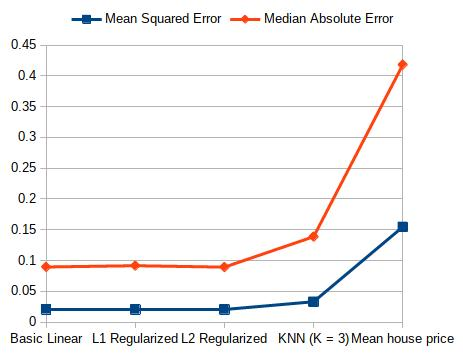
\includegraphics[width=\linewidth]{images/errors.jpg}
\captionof{figure}{Error rates}
\end{minipage}
\hfill
\begin{minipage}{0.49\linewidth}
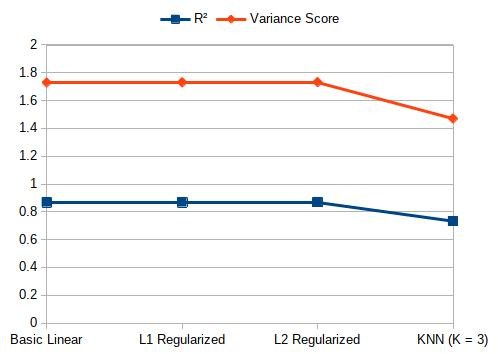
\includegraphics[width=\linewidth]{images/scores.jpg}
\captionof{figure}{$R^2$ and variance score}
\end{minipage}
      \hfill %extra line for space
\end{center}




\section{Conclusion}
The baseline has some divergent results. Both $R^2$ and VS are negative scores. This is caused by the arbitrarily prediction of the baseline for each sample. Looking at the numerator, it shows that this number can get quite large when a prediction is far off the true value. This value is then deducted from 1, which causes it to be a negative value. The same applies to the VS.\\

All of the models have a significantly better performance than the baseline model. This means that they have actually learned how to predict the prices instead of just randomly guessing. In between the models there are some interesting relations. There doesn’t seem to be much difference between the linear models with and without regularization. This may be the case because the linear model is not overfitting. In this case regularization would not be very useful. It is also possible that the model is overfitting, but the predicted prices are still quite accurate. Because most of the house prices lie in the same price range, it could still predict most of the prices around their actual price. \\

Overall, the linear regression models seem to perform slightly better than the kNN model. Because most of the data has a sale price around the mean, linear regression actually predicts the sale price quite accurate. kNN still has a good performance compared to the baseline, with approximately 5 times less (mean squared) error. 


%references page
\clearpage
\bibliographystyle{plain}
\bibliography{references}

\end{document}